% ============= setup ============= %
% ======== package ======== %
\documentclass[mathserif]{beamer}
\usepackage{xeCJK}
\usepackage{graphicx}
\usepackage{xcolor}
\usepackage{setspace}
\usepackage{newtxmath}

% ======== font ======== %
\setCJKmainfont{Taipei Sans TC Beta}
\setCJKsansfont{Taipei Sans TC Beta}
\AtBeginDocument{%
    \DeclareSymbolFont{pureletters}{OML}{cmm}{m}{it}%
    \SetSymbolFont{pureletters}{bold}{OML}{cmm}{b}{it}%
}
\hypersetup{
    colorlinks=true,
    linkcolor=black,
    urlcolor=blue
}

% ======== theme ======== %
\renewcommand{\baselinestretch}{1.25}
\usetheme{Madrid}
\usecolortheme{crane}
\setbeamertemplate{items}[circle]
\setbeamertemplate{section in toc}{\inserttocsectionnumber.~\inserttocsection}
\AtBeginSection[]{
    \begin{frame}
        \vfill
        \centering
        \begin{beamercolorbox}[sep=8pt,center,shadow=true,rounded=true]{title}
            \usebeamerfont{title}\insertsectionhead\par%
        \end{beamercolorbox}
        \vfill
    \end{frame}
}

% ======== data ======== %
\title{Git \& Github 簡介}
\author{temmie}
\date{}

% ============= setup ============= %

\begin{document}

\begin{frame}
    \titlepage
\end{frame}

\begin{frame}
    \tableofcontents
\end{frame}

\section{Git}

\begin{frame}
    \frametitle{什麼是 Git}
    \begin{itemize}
        \item Git 是一種用來管理軟體版本的工具
        \item 目前許多開源的大型專案都保存在線上的 Git 服務
        \item 例如 Github
    \end{itemize}
\end{frame}

\begin{frame}
    \frametitle{安裝 Git - Windows}
    \begin{itemize}
        \item 到 \textbf{Configuring the terminal...} 時
        \item 選擇 \textbf{Use Windows' default console window}
        \item 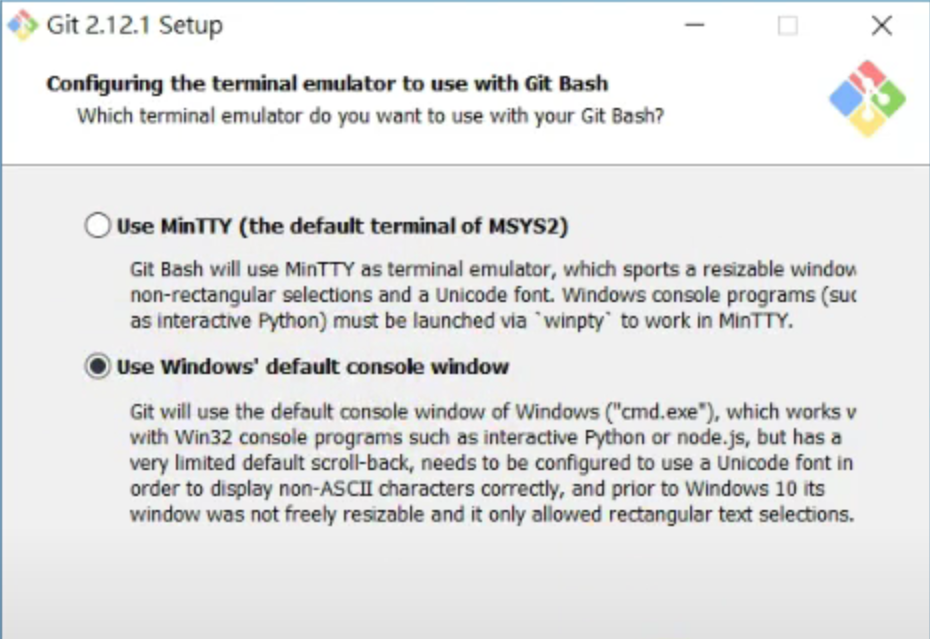
\includegraphics[width=8.0cm]{img/download.jpg}
    \end{itemize}
\end{frame}

\begin{frame}
    \frametitle{安裝 Git - Windows}
    \begin{itemize}
        \item 進入終端機
        \item 打指令\ {\color{red}git},確認是否跑出正常的訊息
    \end{itemize}
\end{frame}

\begin{frame}
    \frametitle{Git 初始化}
    \begin{itemize}
        \item {\color{red}cd} 進去要做為儲存庫的資料夾
        \item 輸入\ {\color{red}git init}
        \item 初始化只需要做一次
    \end{itemize}
\end{frame}

\begin{frame}
    \frametitle{Git 暫存檔案}
    \begin{itemize}
        \item 輸入\ {\color{red}git add [檔案名稱 / 路徑]}
        \item 可以將檔案都加入暫存庫
    \end{itemize}
\end{frame}

\begin{frame}
    \frametitle{Git 紀錄檔案}
    \begin{itemize}
        \item 輸入\ {\color{red}git commit -m [紀錄訊息]}
        \item 可以將暫存庫裡面的檔案紀錄到 git 中
    \end{itemize}
\end{frame}

\section{Github}

\begin{frame}
    \frametitle{Github}
    \begin{itemize}
        \item Github 是一個 Git 為基礎的網路服務平台
        \item<2-> 如果不想要打酷酷的指令的話,可以下載 \href{https://desktop.github.com/}{Github Desktop}
    \end{itemize}
\end{frame}

\begin{frame}
    \frametitle{Github CLI}
    \begin{itemize}
        \item Github CLI 是本地與雲端的橋樑
        \item 可以在本地直接操控雲端的檔案
        \item 也可以在本定直接下載雲端的檔案
    \end{itemize}
\end{frame}

\begin{frame}
    \frametitle{Github CLI -\ 指令}
    \begin{itemize}
        \item {\color{red}gh auth login},照著它給的指令做
        \item<2-> {\color{red}gh repo create},在本地端創建 Github 的儲存庫
        \item<3-> {\color{red}gh repo clone [作者名稱]/[儲存庫名稱]},下載儲存庫檔案
    \end{itemize}
\end{frame}

\begin{frame}
    \frametitle{Github 上傳檔案(初始設定)}
    \begin{itemize}
        \item {\color{red}git remote add [儲存庫簡稱(自取)] [Github 上面的連結]}
        \item {\color{red}git push -u [儲存庫簡稱] main}
    \end{itemize}
\end{frame}

\begin{frame}
    \frametitle{Github 上傳檔案)}
    \begin{itemize}
        \item {\color{red}git add .}
        \item {\color{red}git commit -m "[你的 commit 訊息]"}
        \item {\color{red}git push}
    \end{itemize}
\end{frame}

\end{document}